% !TeX program = pdflatex
% !TeX TS-program = pdflatex
% !TeX TXS-program:compile = txs:///pdflatex/

% !BIB program = biber
% !BIB TS-program = biber
% !TeX TXS-program:bibliography = txs:///biber




\documentclass{beamer}
\usepackage{import}
%\bibliography{Library}
\input    {0_0_Preamble/Preamble_Poster}
\input    {0_0_Preamble/Preamble_BibLaTeX_AER_Poster}  
%\input{0_0_Preamble/Preamble_BibLaTeX_APA}
%\usepackage[backend=biber,natbib=true,style=numeric]{biblatex}
\addbibresource{Library.bib}
\subimport{0_0_Preamble/}{Preamble_Fonts_Charter_FiraSans}
\input    {0_0_Preamble/Preamble_Sansserif_math}
\usepackage{tikz}
\usepackage{float}

%\bibliography{Library}




%%%%%%%%%%%%%%%%%%%%%%%%%%%%%%%%%%%%%%%%%%%%%%%%%%%
%%  DOCUMENT-SPECIFIC ADDITIONS TO THE PREAMBLE  %%
%%%%%%%%%%%%%%%%%%%%%%%%%%%%%%%%%%%%%%%%%%%%%%%%%%%


\newlength{\blockOne}
\newlength{\blockTwo}
\newlength{\blockThree}
\newlength{\blockFour}

% Vertical positions
\setlength{\blockOne}  { 15.50cm} 
\setlength{\blockTwo}  { 47.25cm}
\setlength{\blockThree}{ 75.75cm}
\setlength{\blockFour} {120.00cm}

\title{\firasemibold  The steeper 1/f slope of MEG power spectrum is associated with stronger gamma synchrony, measured via inter-trial phase coherence (ITPC) \\ in the 40-Hz auditory steady-state response}

% (\email{daniel.borek@ugent.be})
% \author{%
% 	 Daniel Borek,\inst{1} \and
% 	 Gang Chen,\inst{2} \and
% 	Giovanni Pellegrino,\inst{3} \and
% 	Giorgio Arcara\inst{3} \and
% 	Daniele Marinazzo\inst{1}
% } %Author(s)

  

% \institute{%
% 	\inst{1} Department of Data Analysis, Faculty of Psychology and Educational Sciences, Ghent, Belgium ;
% 	\and
% 	\inst{2}\,National~Institutes~of~Health,~Bethesda,~MD;
% 	\and
% 	\inst{3}\,IRCCS~San~Camillo~Hospital,~Venice,~Italy%
% } %Institution(s)

% \newcommand{\affilindicator}[1]{\textsuperscript{#1}}

% Then your original code should work:
\author{%
	 Daniel Borek,\affilindicator{a}
	 Gang Chen,\affilindicator{b} 
	Giovanni Pellegrino,\affilindicator{c}
	Giorgio Arcara\affilindicator{c} and
	Daniele Marinazzo\affilindicator{a}
}

\institute{%
	\affilindicator{a}\,Department of Data Analysis, Faculty of Psychology and Educational Sciences, Ghent, Belgium ;
	\affilindicator{b}\,National~Institutes~of~Health,~Bethesda,~MD;
	\affilindicator{c}\,IRCCS~San~Camillo~Hospital,~Venice,~Italy%
}


\usepackage{xspace}
\newcommand{\balA}[1][1]{BAL$^\mathup{I}_{#1:#1}$\xspace}
\newcommand{\unbalA}[1][n]{UNBAL$^\mathup{I}_{1:#1}$\xspace}
\newcommand{\balB}[1][1]{BAL$^\mathup{II}_{#1:#1}$\xspace}
\newcommand{\unbalB}[1][n]{UNBAL$^\mathup{II}_{#1:1}$\xspace}

\newcommand{\mynum}[1]{\scalebox{1.075}{\firasemibold#1}}




%%%%%%%%%%%%%%%%%%%%%
%%  DOCUMENT BODY  %%
%%%%%%%%%%%%%%%%%%%%%


\begin{document}


\begin{frame}[t]	% Entire poster is one large frame


%\TPshowboxestrue


%%%%%%%%%%%%%%%%%%%%%%%%%%%%%%  COLUMN 1  %%%%%%%%%%%%%%%%%%%%%%%%%%%%%%
\TPshowboxesfalse

\begin{textblock*}{\colwidth}(\leftmargin, \blockOne+3cm)  % Add 3cm below original position

\begin{alertblock}{%
	\begin{minipage}[b]{55pt}
		\RaggedRight
	
	\end{minipage}%
	\begin{minipage}[b]{0.9\colwidth}
		Hypothesis.\;
		{\mdseries 	We  explored whether a steeper slope of the 1/f  PSD component (i.e., a larger spectral exponent) in MEG signals is associated with higher auditory steady-state response (ASSR) synchrony, as measured by inter-trial phase coherence (ITPC) during 40 Hz auditory stimulation.
		}
	\end{minipage}%
}
\end{alertblock}

\begin{parblock}{Introduction}

	\begin{itemize}
		\item  Power spectral density (PSD) of electrophysiological activity  may be parametrized by  oscillatory components  and aperiodic component, where the power of the signal decay with a 1/f power law
		\item The timescale and magnitude of this aperiodic activity can be described by the slope and offset of this 1/f decay \citep{donoghue2020a}
		



	\end{itemize}

\end{parblock}

\end{textblock*}
\TPshowboxestrue
%%%%%%%%%%%%%%%%%%%%%%%%%%%%%%  COLUMN 2 & 3  %%%%%%%%%%%%%%%%%%%%%%%%%%%%%%
% \begin{textblock*}{2\colwidth+\colsep}(\leftmargin+\colwidth+\colsep, \blockOne)

% 	\begin{alertblock}{%
% 		\begin{minipage}[b]{55pt}
% 			\RaggedRight
% 			\noindent\hspace{-10pt}\VeryHuge 1
% 		\end{minipage}%
% 		\begin{minipage}[b]{2\colwidth+\colsep-125pt}
% 			Spectral Parametrization.\;
% 			{\mdseries Mean values of parameters describing the aperiodic part od  spectral power across different regions (right hemishpere).}\;
% 			(A)~{\mdseries Offset.}\;
% 			(B)~{\mdseries Exponent.}
% 		\end{minipage}%
% 	}
% 	\begin{minipage}[t]{.49\linewidth}
% 		\begin{figure}
% 		\begin{center} \hspace*{-10.35cm}
% 	  \includegraphics[scale=2.25]{figures/offset.png}
% 	\end{center}
% 	 \end{figure}
% 	\end{minipage} 
% 	\begin{minipage}[t]{.49\linewidth}
% 		\begin{figure}
% 		\begin{center} \hspace*{-10.35cm}
% 	  \includegraphics[scale=2.25]{figures/exponent.png}
% 	\end{center}
% 	 \end{figure}
% 	\end{minipage}


% \end{alertblock}
% \end{textblock*}

\TPshowboxesfalse

\begin{textblock*}{0.9\colwidth}(\leftmargin+\colwidth+\colsep, \blockOne)
	\begin{block}{~}
		%\vspace{-0.333333\baselineskip}
	% 	\begin{figure}
	% 		\begin{center}
	% % TODO #1 Make my own figure with the right dimensions
	% 	  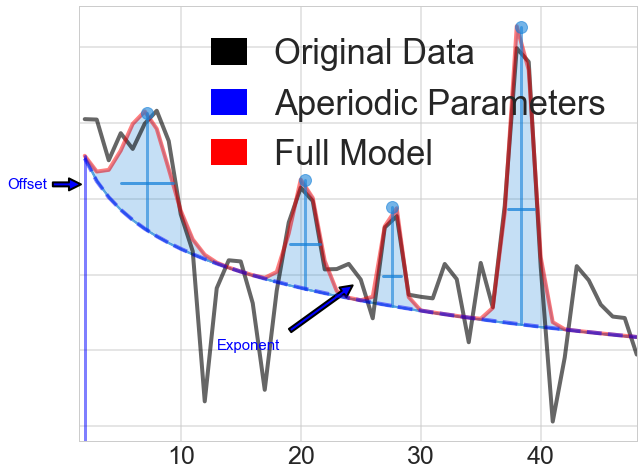
\includegraphics[scale=0.7]{figures/Schema.png}
	% 	\end{center}
		 %\end{figure}
		\begin{itemize}

			\item  Simplified formula  describing 1/f component  of the  PSD  of the signal: $L(f) = b - \log(k + f^\chi)$;  The exponent ${\chi}$ is related to the negative slope of the power spectrum in log-log space, that is, the inverse relationship between power and frequency;  The offset $b$ describe the uniform shift in power across frequencies
		\item These parameters are most likely governed by waxing and waning of oscillatory components, and can be associated to biological mechanisms (e.g. excitation:inhibition balance as summed by \citep{waschke2021}, cognitive processes, and group differences). 
		
			\item  Graphical relationship of spectral power and offset and exponent (from \citep{hill2022})
  
		\end{itemize}
	

		\begin{figure}
		\begin{center}
	  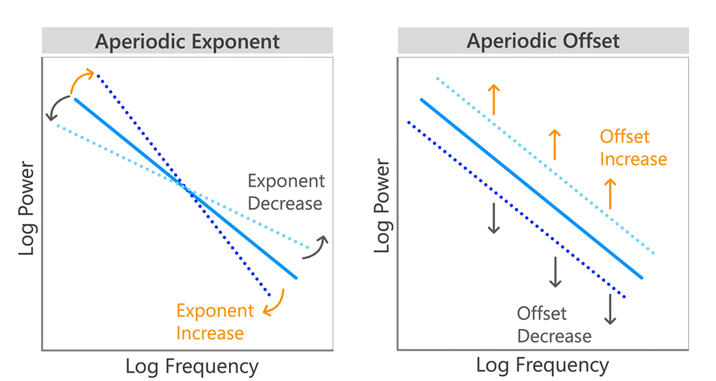
\includegraphics[scale=2.6]{figures/Aperiodic2.jpg}
	\end{center}
	 \end{figure}

	\end{block}
\end{textblock*}

\TPshowboxestrue
\begin{textblock*}{1.1\colwidth}(\leftmargin+1.9\colwidth+2\colsep,  \blockOne+3cm)

	\begin{alertblock}{%
		\begin{minipage}[b]{55pt}
			\RaggedRight
			\noindent\hspace{-10pt}\VeryHuge 1
		\end{minipage}%
		\begin{minipage}[b]{0.9\linewidth+\colsep-125pt}
			Spectral Parametrization.\;
			{\mdseries Mean values \mbox{of} \mbox{estimated} \mbox{exponent} and offset describing the 1/f part \mbox{of}  \mbox{spectral} \mbox{power} across different regions (right hemisphere). }
		\end{minipage}%
	}
	\begin{minipage}[t]{.99\linewidth}
		\begin{figure}
		\begin{center} \hspace*{-1.0cm}
	  \includegraphics[width=1.1\linewidth]{figures/combined.png}
	\end{center}
	 \end{figure}
	\end{minipage} 



\end{alertblock}
\end{textblock*}
%%%%%%%%%%%%%%%%%%%%%%%%%%%%%%  COLUMN 2  %%%%%%%%%%%%%%%%%%%%%%%%%%%%%%







%%%%%%%%%%%%%%%%%%%%%%%%%%%%%%  BOX 2  %%%%%%%%%%%%%%%%%%%%%%%%%%%%%%


\begin{textblock*}{2\colwidth+\colsep}(\leftmargin, \blockTwo)

\begin{alertblock}{%
	\begin{minipage}[b]{55pt}
		\RaggedRight
		\noindent\hspace{-10pt}\VeryHuge 2
	\end{minipage}%
	\begin{minipage}[b]{2\colwidth+\colsep-125pt}
		Relationship between the slope (parametrized by exponent and the estimated ITPC).\;
		{\mdseries Figure on the left:  Relationship between Spectral Exponent (z-scored) and ITPC across selected ROIs. Red line indicates linear fit. Data points colored by subject.}
	\end{minipage}%
}
\begin{minipage}[t]{.89\linewidth}
	\begin{figure}
	\begin{center} 
    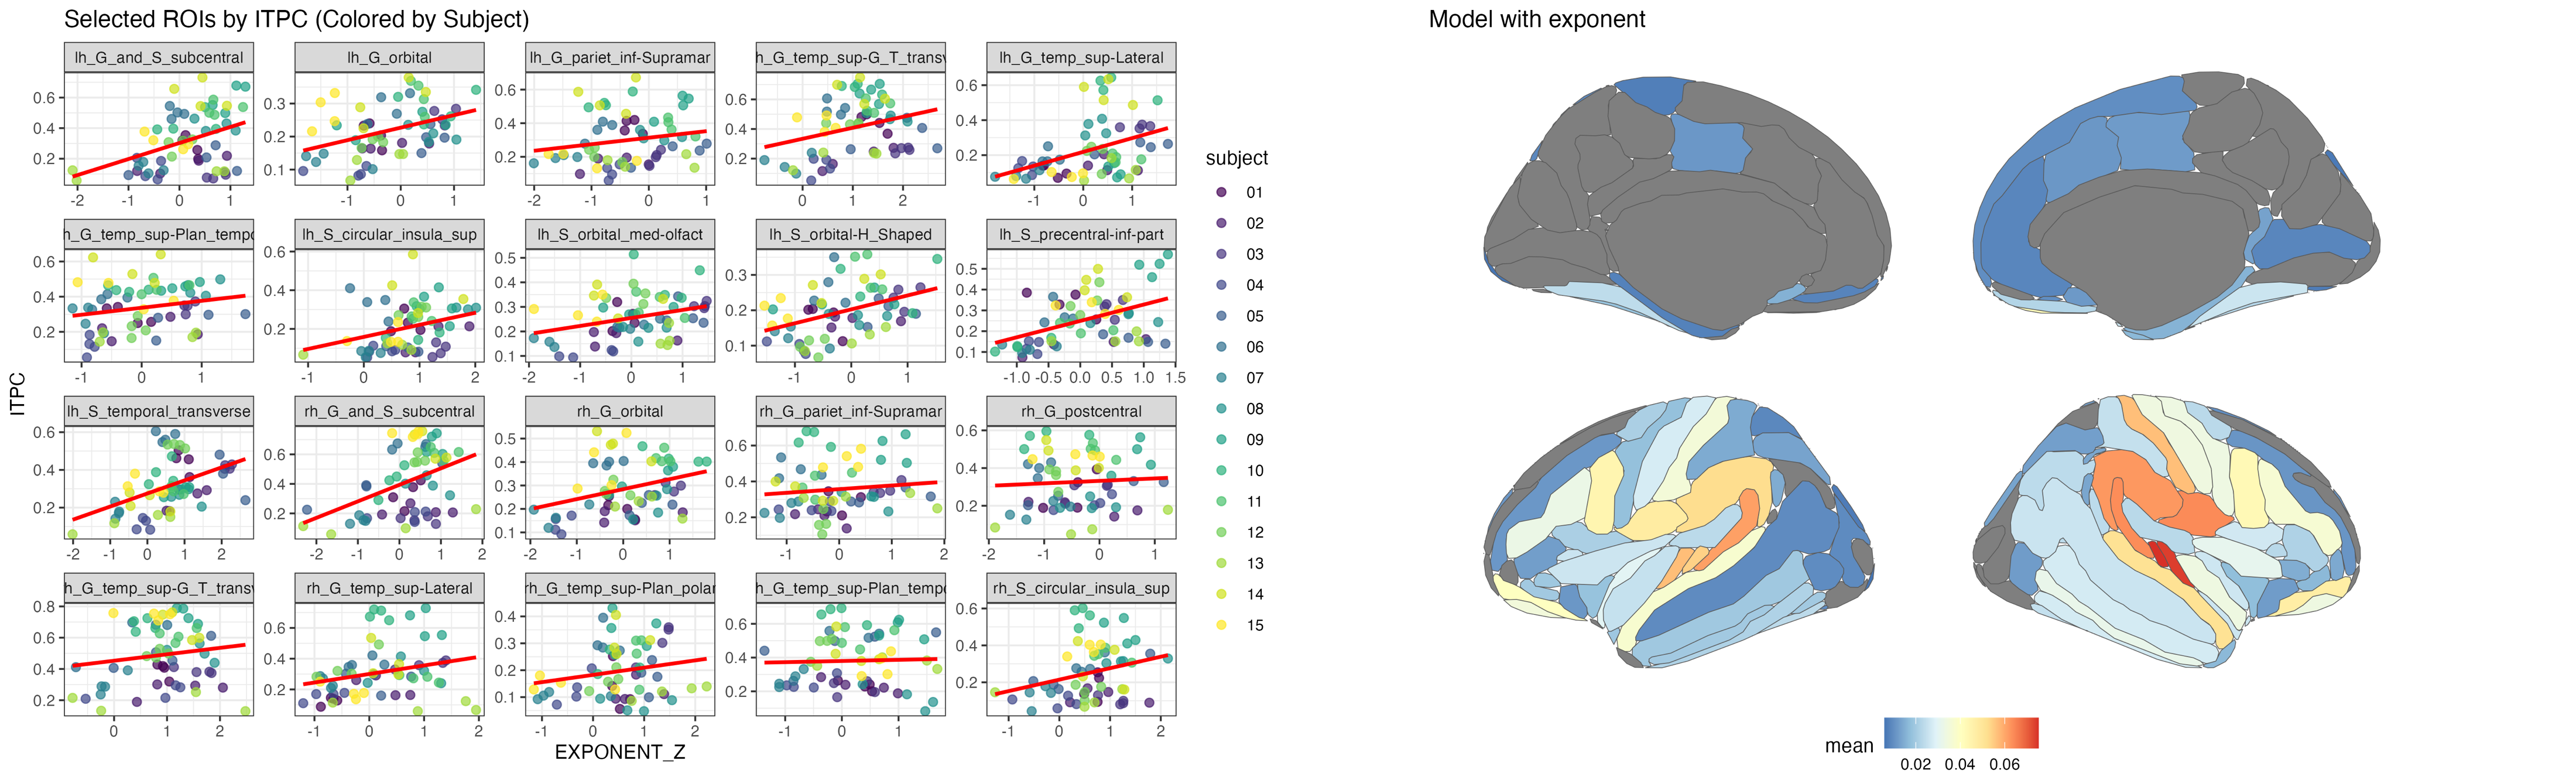
\includegraphics[width=1.10\linewidth,clip]{figures/result.png}%


\end{center}
 \end{figure}
\end{minipage}%

\end{alertblock}

\end{textblock*}





%%%%%%%%%%%%%%%%%%%%%%%%%%%%%%  BOX 3  %%%%%%%%%%%%%%%%%%%%%%%%%%%%%%






\TPshowboxesfalse

\begin{textblock*}{\colwidth}(\leftmargin+2\colwidth+2\colsep, \blockTwo-150pt)


% 	\begin{parblock}{Synchronisation}

% 			\item Synchronization of brain activity in the gamma frequency is a hallmark of brain function, and an indicator of malfunctioning\citep{pellegrino2019}.
%    \item Auditory stimulation in the gamma range is a reliable way to experimentally investigate this phenomenon, looking at auditory steady-state responses  (ASSR), the effect of entrainment of brain activity to the frequency and phase  of external auditory stimuli.  
% 		 \item ASSR are usually investigated by looking at the intertrial phase coherence (ITPC) \citep{pellegrino2019}.	
		



% 	\end{itemize}

% \end{parblock}

	\begin{block}{~}
		\begin{itemize}
		
			\item Synchronization of brain activity in the gamma frequency is a hallmark of brain function, and an indicator of malfunctioning\citep{pellegrino2019}.
   \item Auditory stimulation in the gamma range is a reliable way to experimentally investigate this phenomenon, looking at auditory steady-state responses  (ASSR), the effect of entrainment of brain activity to the frequency and phase  of external auditory stimuli.  
		 \item ASSR are usually investigated by looking at the intertrial phase coherence (ITPC) \citep{pellegrino2019}.	
		\end{itemize}	
		\end{block}
		

\end{textblock*}
% \begin{textblock*}{\colwidth}(\leftmargin+2\colwidth+2\colsep, \blockTwo+300pt)
% \begin{alertblock}{%
% 	\begin{minipage}[b]{55pt}
% 		\RaggedRight
	
% 	\end{minipage}%
% 	\begin{minipage}[b]{0.9\colwidth}
% 		Hypothesis.\;
% 		{\mdseries 	We hypothesize that the slope of the 1/f component in the power spectral density of resting-state MEG signals will negatively correlate with auditory steady-state response (ASSR) detectability, as measured by inter-trial phase coherence (ITPC) during auditory stimulation:


% 		}
% 	\end{minipage}%
% }
% \end{alertblock}
% \end{textblock*}



% \begin{textblock*}{\colwidth}(\leftmargin+2\colwidth+2\colsep, \blockTwo+320pt)
% 	% \begin{block}{Data }
% 	% 	\vspace{-0.333333\baselineskip}
	
% 	% 	\begin{itemize}
% 	% 		\item We re-analysed MEG data from  n=15 healthy participants, stimulated with a sound wave modulated at 40 Hz, presented in 180 trials for one second, with the onset of two consecutive trials separated by at least 2 s \citep{pellegrino2019}.
	
%  	% 		\item The data were preprocessed, projected into Destrieux brain atlas 

   
% 	% 	\end{itemize}
% 	% 	\end{block}
% \begin{block}{Data}
%     \vspace{-0.333333\baselineskip}
%     \begin{itemize}
%         \item \textbf{Reanalysis of MEG data} from n=15 healthy participants \citep{pellegrino2019}
%         \item \textbf{Paradigm:} 180 trials of 40-Hz amplitude-modulated auditory stimulation (1s duration, $\geq$2s inter-trial interval)
%         \item \textbf{Preprocessing:} Source reconstruction to 148 cortical regions (Destrieux atlas)
%     \end{itemize}
% \end{block}

% \end{textblock*}

%%%%%%%%%%%%%%%%%%%%%%%%%%%%%%  COLUMN 1  %%%%%%%%%%%%%%%%%%%%%%%%%%%%%%
\begin{textblock*}{\colwidth}(\leftmargin, \blockThree-150pt)

% 	\begin{block}{Methods }
% 		\vspace{-0.333333\baselineskip}
% 		\begin{itemize}
%        \item 	The PSD  of the spectrum were  computed for 1s second pre-stimulus period and stimulation period for each trial (and averaged later) and for each region. The slope and exponent were computed  using specparam toolbox \citep{donoghue2020a}.

% 			\item ITPC was computed, the value averaged in the intervals $[-500,-200]$ ms for prestimuli and  $[400, 700]$ ms after sound onset for each of the regions using the wavelet approach described in \citep{pellegrino2019}.
%    \item The influence of the stimulus and the exponent on the ITPC were tested by modelling the different relationships with an integrative Bayesian Multilevel Model \citep{chen2019a} 
%    \item This methods allows for better integration of the spatial information and control of multiplicity avoding information loss of univariate approach followed by the correction for multiple testing.
%  \item Effect estimation and region-level inferences  are based on posterior distributions of group differences. 
% 		\end{itemize}

% 		Following models were tested:
% 		\begin{itemize}
% 			\item[\mynum{1}] ITPC $\thicksim$ S (Stimulus)
% 			\item[\mynum{2}] ITPC $\thicksim$ Exponent + Stimulus
% 			\item[\mynum{3}] Exponent $\thicksim$  Stimulus
% 			\item[\mynum{5}] Offset $\thicksim$ Stimulus
% \item  For investigation of the the relationship we fit the model 
% $${\small \text{ITPC}_{\text{stim}} \sim 1 + \text{exponent}_z + (1 + \text{exponent}_z \mid \text{subject}) + (1 \mid \text{ROI})}$$ 
% with z-scored Exponent. The model was fitted using the \texttt{brms} package and \citep{chen2019a}.
% 		\end{itemize}

% 	\end{block}



\begin{block}{ Data and Methods}
    \vspace{-0.333333\baselineskip}

	\textbf{Data:}
    \begin{itemize}
     \item \textbf{n=15 healthy participants;} In block 180 trials of 40-Hz auditory stimulation (1s duration) \citep{pellegrino2019}
        \item Source-reconstructed MEG data from 148 cortical regions (Destrieux atlas)
    \end{itemize}
    
    \textbf{Spectral Parameterization:}
    \begin{itemize}
        \item PSD computed for 1s pre-stimulus and stimulus periods per trial/region
        \item Exponent and offset extracted using \texttt{specparam} \citep{donoghue2020a} from 3-45 Hz range
    \end{itemize}
    
    \textbf{Phase-Locking Measurement:}
    \begin{itemize}
        \item ITPC computed via Morlet wavelets at 40 Hz \citep{pellegrino2019}
        \item Baseline: $[-500,-200]$ ms; Stimulation: $[400,700]$ ms post-onset
    \end{itemize}
    
    \textbf{Statistical Analysis:}
    \begin{itemize}
        \item \textbf{Bayesian multilevel modeling} via Region-Based Analysis (RBA) \citep{chen2019a}, accounts for spatial structure and multiple comparisons through hierarchical pooling
        \item Posterior distributions quantify effect uncertainty across 148 regions
    \end{itemize}
    
    \textbf{Models tested:}
    \begin{itemize}
        \item[\mynum{1}] ITPC $\thicksim$ Stimulus (entrainment effect)
        \item[\mynum{2}] Exponent $\thicksim$ Stimulus (stability test)
        \item[\mynum{3}] Offset $\thicksim$ Stimulus
    \end{itemize}
    
    \textbf{Primary model (exponent-ITPC relationship):}
    $${\small \text{ITPC}_{\text{stim}} \sim 1 + \text{exponent}_z + (1 + \text{exponent}_z \mid \text{subject}) + (1 \mid \text{ROI})}$$
    where exponent$_z$ is within-subject z-scored. Fitted using \texttt{brms} package.
\end{block}

\end{textblock*}





%%%%%%%%%%%%%%%%%%%%%%%%%%%%%%  COLUMN 3  %%%%%%%%%%%%%%%%%%%%%%%%%%%%%%
\begin{textblock*}{\colwidth}(\leftmargin+\colwidth+\colsep, \blockThree-150pt)

	\begin{block}{~}
		\vspace{-0.333333\baselineskip}
		
	\end{block}
\end{textblock*}


\begin{textblock*}{\colwidth}(\leftmargin+\colwidth+\colsep, \blockThree-150pt)

	% \begin{block}{Results {\mdseries(Box 2)}}
	% 	\vspace{-0.333333\baselineskip}
	% 	\begin{itemize}
	% 		\item Exponent and the offset of the spectrum are different across the brain (Box 1); 
	% 		\item Strong effect of the stimulus (S) on the ITPC (contrast baseline-stimulus), in areas like the auditory regions, but also in temporal lobe, inferior part of primary sensory-motor regions and inferior frontal regions; negative values indicate higher ITPC during stimulation.
	
	% 		\item No particular evidence was found for the model $Exponent \thicksim Stimulus$, namely the stimulation did not influence the exponent per se.
	% 		\item No significant evidence was found for any of the models involving the Offset either as a predicted variable, and as a predictor, suggesting a marginal role for it in the auditory entrainment.	
	% 		 \item  Looking for a raw relationship between exponent and ITPC shows a positive relationship between the Exponent and the ITPC, suggesting that higher Exponent is associated with higher ITPC, i.e. higher synchrony during stimulation.
	% 		\item Hierarchical Bayesian modelling allows to estimate the posterior distribution of the coefficients, which can be used to assess the significance of the effect.  It also uses pooling of the data across subjects and regions. The posterior distribution of the coefficient is shown in the Box 2, on the right.		
	
			
	% 	\end{itemize}	
	% 	\end{block}
		
\begin{block}{Results}
	\vspace{-0.333333\baselineskip}
	
	\textbf{Spatial Distribution \& Stability:}
	\begin{itemize}
		\item Exponent and offset varied systematically across brain regions (Box 1)
		\item Exponent remained stable during auditory stimulation (no evidence for Stimulus effect)
		\item Offset showed no systematic changes across conditions
	\end{itemize}
	
	\textbf{ITPC Response to Auditory Stimulation:}
	\begin{itemize}
		\item Strong stimulus effect on ITPC (baseline vs.\ stimulation) in auditory cortex, temporal lobe, inferior sensorimotor regions, and inferior frontal regions
		\item Right hemisphere showed somewhat stronger effects
	\end{itemize}
	
	\textbf{Exponent-ITPC Relationship:}
	\begin{itemize}
		\item Positive relationship between exponent and ITPC during stimulation 
		\item Steeper spectral slopes associated with stronger phase-locking
		\item Regional specificity: Strongest effects in right superior temporal gyrus, temporal pole, insula, and inferior frontal regions---overlapping with regions showing robust ASSR responses
		\item Offset showed no significant relationship with ITPC
	\end{itemize}
	
	\textbf{Statistical Approach:}
	\begin{itemize}
		\item Bayesian multilevel modeling accounts for spatial structure and multiple comparisons through hierarchical pooling
		\item Posterior distributions and $P^+$ quantify uncertainty in estimates
	\end{itemize}
\end{block}

\end{textblock*}


%%%%%%%%%%%%%%%%%%%%%%%%%%%%%%  COLUMNS 1 + 2  %%%%%%%%%%%%%%%%%%%%%%%%%%%%%%


\begin{textblock*}{2\colwidth+\colsep}(\leftmargin, \blockFour)

\begin{block}{~}
\end{block}

\end{textblock*}


%%%%%%%%%%%%%%%%%%%%%%%%%%%%%%  COLUMN 1  %%%%%%%%%%%%%%%%%%%%%%%%%%%%%%


\begin{textblock*}{\colwidth}(\leftmargin+2\colwidth+2\colsep, \blockThree -460pt)
\noindent\rule{\linewidth}{0.5pt}

% \begin{block}{Conclusion}
% \vspace{-0.333333\baselineskip}
% \begin{itemize}
% 	\item The differences observed might simply reflect increased "noise" in the time-domain signal, potentially diminishing SNR and synchrony. Alternatively, from a biological perspective, this effect might be linked with excitation-inhibition balance, which influence both synchrony measures and spectral slope.
% 	\item The effects of the aperiodic slope on the estimation of the instantaneous phase and the ITPC \citep{samaha2022} could be \mbox{considered} in further analysis  as well as a effect of higher gamma power for aperiodic slope  estimation.
% \end{itemize}	
% \emph{Acknowledgments:} For visualising the results ggseg \mbox{library} was
% used \citep{mowinckel2020}
% \end{block}

\begin{block}{Conclusion}
	\vspace{-0.333333\baselineskip}
	
	\textbf{Main Finding:}
	\begin{itemize}
		\item Steeper spectral slopes associated with stronger gamma phase-locking, particularly in auditory and temporal regions showing robust ASSR responses
	\end{itemize}
	
	\textbf{Two Possible Mechanisms:}
	\begin{itemize}
		\item \textbf{Biological:} Both measures may reflect E/I balance---stronger inhibitory tone (steeper slope) provides temporal scaffolding for precise synchronization \citep{waschke2021}
		\item \textbf{Methodological:} Spectral slope influences phase estimation reliability and SNR \citep{vandiepen2018CaveatsObservingInterTrial, samaha2022}

		\item Regional specificity and exponent stability suggest biological contribution, though methodological confounding cannot be fully ruled out
	\end{itemize}
	
	\textbf{Implications:}
	\begin{itemize}
		\item Exploratory findings ($n=15$) warrant replication in larger samples
		\item Combined spectral-oscillatory measures may enhance sensitivity to circuit dysfunction
		\item Future work should distinguish biological from methodological contributions through controlled simulations and clinical validation
	\end{itemize}
\end{block}

\end{textblock*}


%%%%%%%%%%%%%%%%%%%%%%%%%%%%%%  COLUMN 2  %%%%%%%%%%%%%%%%%%%%%%%%%%%%%%


\begin{textblock*}{\colwidth}(\leftmargin+\colwidth+\colsep, \blockFour)

\begin{block}{~}
\vspace{-0.333333\baselineskip}

\end{block}

\end{textblock*}


%%%%%%%%%%%%%%%%%%%%%%%%%%%%%%  COLUMN 3  %%%%%%%%%%%%%%%%%%%%%%%%%%%%%%


\begin{textblock*}{\colwidth}(\leftmargin+2\colwidth+2\colsep, \blockThree+465pt)

\begin{block}{\refname}
\vspace{-0.333333\baselineskip}
\setlength{\bibhang}{0pt}
\setlength{\bibsep}{0\baselineskip}
\renewcommand*{\bibfont}{\sffamily\small\baselineskip25.9pt}
\renewcommand*{\bf}{\bfseries}
\color{SpotColor}
\begin{refcontext}[sorting=nyt]
	% Sort BIBLIOGRAPHY by alphabet (while CITATIONS are sorted by year)
\printbibliography[heading=none]
\end{refcontext}
%% Only when using BibTeX instead of BibLaTeX ==>
%\bibliographystyle{0_0_Preamble/aea_doi_initials}
%\renewcommand{\harvardand}{\&}
%\bibliography{Library}
%% <==
\end{block}

\end{textblock*}


\end{frame}


\end{document}